\documentclass[border=2mm]{standalone}
\usepackage{tikz}
\usepackage{pgfplots}
\usepackage{amsmath}
\usepackage{xcolor}
\usetikzlibrary{shapes.geometric, arrows, positioning, decorations.pathreplacing, patterns, shadows, calc}

\pgfplotsset{compat=1.17}

% Define colors
\definecolor{primaryblue}{RGB}{51, 122, 183}
\definecolor{successgreen}{RGB}{92, 184, 92}
\definecolor{warningyellow}{RGB}{240, 173, 78}
\definecolor{dangerred}{RGB}{217, 83, 79}
\definecolor{lightgray}{RGB}{248, 248, 248}
\definecolor{darkgray}{RGB}{51, 51, 51}

\begin{document}

% ---
% Figure 1: XAI Analysis Workflow
% ---
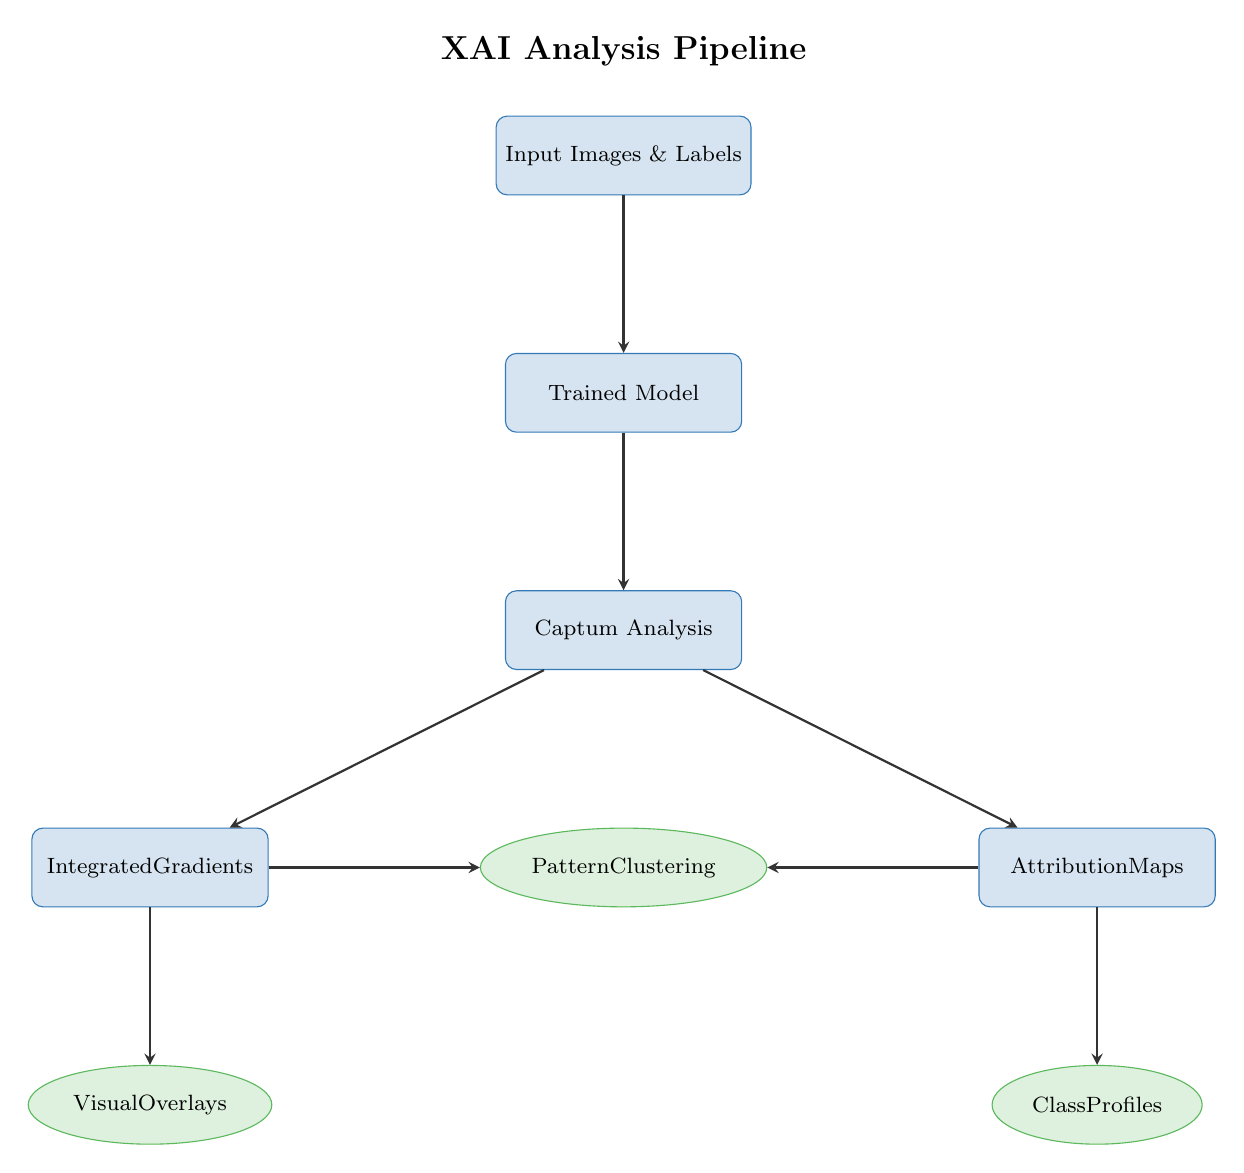
\begin{tikzpicture}[
    node distance=2cm and 3cm,
    process/.style={rectangle, rounded corners, minimum width=3cm, minimum height=1cm, text centered, draw=primaryblue, fill=primaryblue!20, font=\footnotesize},
    decision/.style={diamond, minimum width=2cm, minimum height=1cm, text centered, draw=warningyellow, fill=warningyellow!20, font=\footnotesize},
    output/.style={ellipse, minimum width=2.5cm, minimum height=1cm, text centered, draw=successgreen, fill=successgreen!20, font=\footnotesize},
    arrow/.style={thick,->,>=stealth, draw=darkgray}
]

\node (input) [process] {Input Images \& Labels};
\node (model) [process, below=of input] {Trained Model};
\node (captum) [process, below=of model] {Captum Analysis};
\node (gradients) [process, below left=of captum] {Integrated\\Gradients};
\node (attribution) [process, below right=of captum] {Attribution\\Maps};
\node (overlay) [output, below=of gradients] {Visual\\Overlays};
\node (profiles) [output, below=of attribution] {Class\\Profiles};
\node (clustering) [output, below=2cm of captum] {Pattern\\Clustering};

\draw [arrow] (input) -- (model);
\draw [arrow] (model) -- (captum);
\draw [arrow] (captum) -- (gradients);
\draw [arrow] (captum) -- (attribution);
\draw [arrow] (gradients) -- (overlay);
\draw [arrow] (attribution) -- (profiles);
\draw [arrow] (gradients) -- (clustering);
\draw [arrow] (attribution) -- (clustering);

\node [above=0.5cm of input, font=\large\bfseries] {XAI Analysis Pipeline};

\end{tikzpicture}

% ---
% Figure 2: Model Comparison Framework
% ---
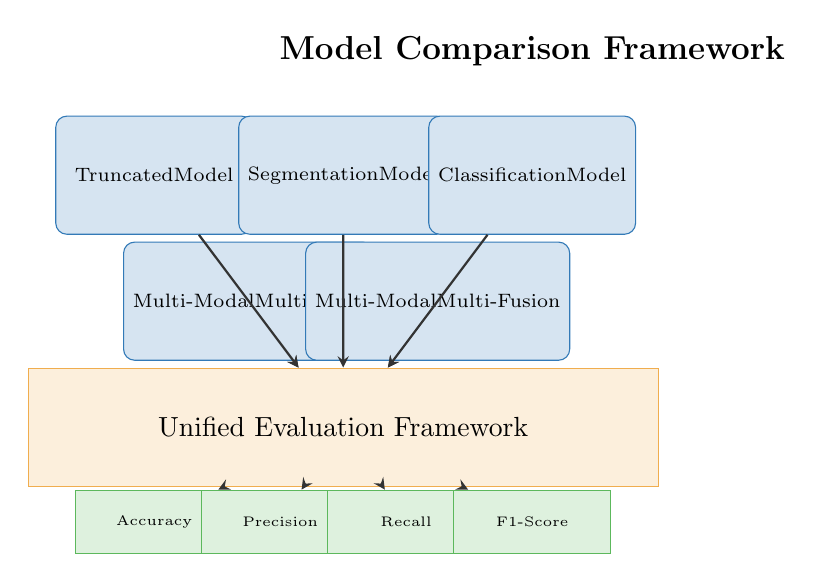
\begin{tikzpicture}[
    scale=0.8,
    model/.style={rectangle, rounded corners, minimum width=2.5cm, minimum height=1.5cm, text centered, draw=primaryblue, fill=primaryblue!20, font=\scriptsize},
    metric/.style={rectangle, minimum width=2cm, minimum height=0.8cm, text centered, draw=successgreen, fill=successgreen!20, font=\tiny},
    arrow/.style={thick,->,>=stealth, draw=darkgray}
]

% Models
\node (truncated) [model] at (0,4) {Truncated\\Model};
\node (segmentation) [model] at (3,4) {Segmentation\\Model};
\node (classification) [model] at (6,4) {Classification\\Model};
\node (multiscale) [model] at (1.5,2) {Multi-Modal\\Multi-Scale};
\node (multifusion) [model] at (4.5,2) {Multi-Modal\\Multi-Fusion};

% Evaluation Framework
\node (evaluation) [rectangle, minimum width=8cm, minimum height=1.5cm, text centered, draw=warningyellow, fill=warningyellow!20] at (3,0) {Unified Evaluation Framework};

% Metrics
\node (accuracy) [metric] at (0,-1.5) {Accuracy};
\node (precision) [metric] at (2,-1.5) {Precision};
\node (recall) [metric] at (4,-1.5) {Recall};
\node (f1score) [metric] at (6,-1.5) {F1-Score};

% Arrows
\foreach \model in {truncated, segmentation, classification, multiscale, multifusion} {
    \draw [arrow] (\model) -- (evaluation);
}

\foreach \metric in {accuracy, precision, recall, f1score} {
    \draw [arrow] (evaluation) -- (\metric);
}

\node [above=0.5cm of classification, font=\large\bfseries] {Model Comparison Framework};

\end{tikzpicture}

% ---
% Figure 3: Binary Classifier Strategy
% ---
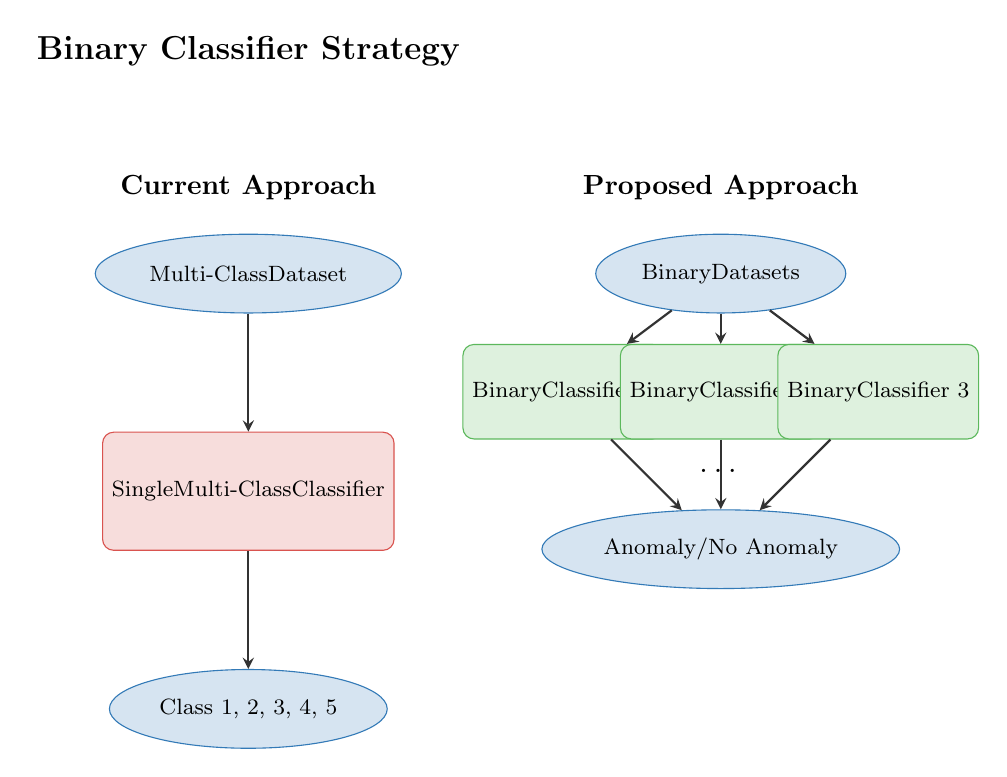
\begin{tikzpicture}[
    node distance=1.5cm and 2cm,
    current/.style={rectangle, rounded corners, minimum width=3cm, minimum height=1.5cm, text centered, draw=dangerred, fill=dangerred!20, font=\footnotesize},
    proposed/.style={rectangle, rounded corners, minimum width=2.5cm, minimum height=1.2cm, text centered, draw=successgreen, fill=successgreen!20, font=\footnotesize},
    data/.style={ellipse, minimum width=2cm, minimum height=1cm, text centered, draw=primaryblue, fill=primaryblue!20, font=\footnotesize},
    arrow/.style={thick,->,>=stealth, draw=darkgray}
]

% Current Approach
\node (current_data) [data] at (0,3) {Multi-Class\\Dataset};
\node (current_model) [current, below=of current_data] {Single\\Multi-Class\\Classifier};
\node (current_output) [data, below=of current_model] {Class 1, 2, 3, 4, 5};

% Proposed Approach
\node (proposed_data) [data] at (6,3) {Binary\\Datasets};
\node (binary1) [proposed] at (4,1.5) {Binary\\Classifier 1};
\node (binary2) [proposed] at (6,1.5) {Binary\\Classifier 2};
\node (binary3) [proposed] at (8,1.5) {Binary\\Classifier 3};
\node (dots) [font=\large] at (6,0.5) {\ldots};
\node (proposed_output) [data] at (6,-0.5) {Anomaly/\\No Anomaly};

% Arrows Current
\draw [arrow] (current_data) -- (current_model);
\draw [arrow] (current_model) -- (current_output);

% Arrows Proposed
\draw [arrow] (proposed_data) -- (binary1);
\draw [arrow] (proposed_data) -- (binary2);
\draw [arrow] (proposed_data) -- (binary3);
\draw [arrow] (binary1) -- (proposed_output);
\draw [arrow] (binary2) -- (proposed_output);
\draw [arrow] (binary3) -- (proposed_output);

% Labels
\node [above=0.3cm of current_data, font=\bfseries] {Current Approach};
\node [above=0.3cm of proposed_data, font=\bfseries] {Proposed Approach};

\node [above=2cm of current_data, font=\large\bfseries] {Binary Classifier Strategy};

\end{tikzpicture}

% ---
% Figure 4: Experiment Tracking Workflow
% ---
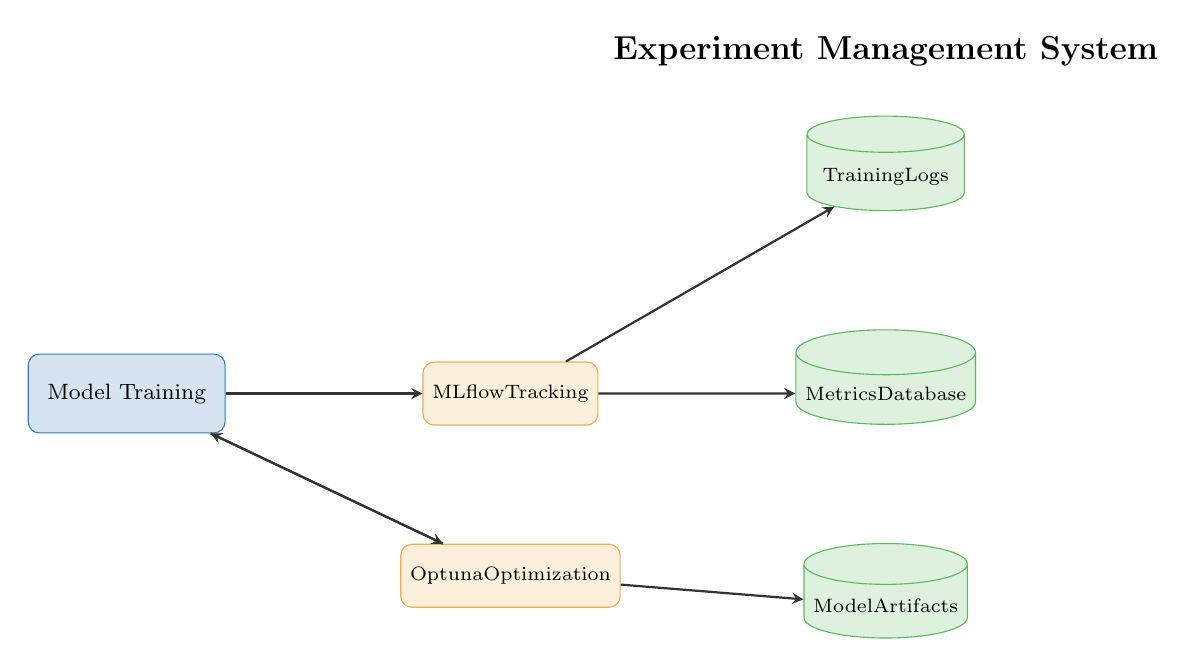
\begin{tikzpicture}[
    node distance=1.5cm and 2.5cm,
    component/.style={rectangle, rounded corners, minimum width=2.5cm, minimum height=1cm, text centered, draw=primaryblue, fill=primaryblue!20, font=\footnotesize},
    tracking/.style={rectangle, rounded corners, minimum width=2cm, minimum height=0.8cm, text centered, draw=warningyellow, fill=warningyellow!20, font=\scriptsize},
    storage/.style={cylinder, shape border rotate=90, aspect=0.25, minimum width=2cm, minimum height=1.2cm, text centered, draw=successgreen, fill=successgreen!20, font=\scriptsize},
    arrow/.style={thick,->,>=stealth, draw=darkgray}
]

\node (training) [component] {Model Training};
\node (mlflow) [tracking, right=of training] {MLflow\\Tracking};
\node (optuna) [tracking, below=of mlflow] {Optuna\\Optimization};
\node (metrics) [storage, right=of mlflow] {Metrics\\Database};
\node (artifacts) [storage, below=of metrics] {Model\\Artifacts};
\node (logs) [storage, above=of metrics] {Training\\Logs};

\draw [arrow] (training) -- (mlflow);
\draw [arrow] (training) -- (optuna);
\draw [arrow] (mlflow) -- (metrics);
\draw [arrow] (mlflow) -- (logs);
\draw [arrow] (optuna) -- (artifacts);
\draw [arrow] (optuna) -- (training);

\node [above=0.5cm of logs, font=\large\bfseries] {Experiment Management System};

\end{tikzpicture}

% ---
% Figure 5: Development Timeline
% ---
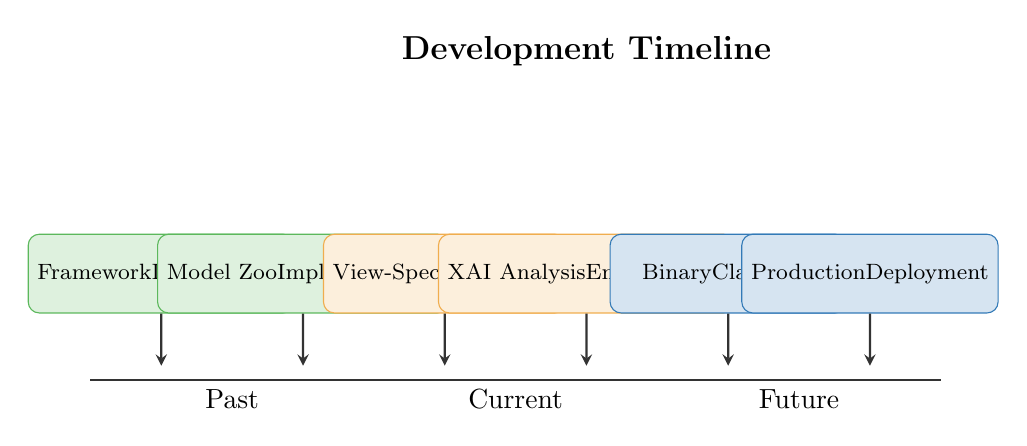
\begin{tikzpicture}[
    scale=0.9,
    phase/.style={rectangle, rounded corners, minimum width=3cm, minimum height=1cm, text centered, font=\footnotesize},
    completed/.style={phase, draw=successgreen, fill=successgreen!20},
    current/.style={phase, draw=warningyellow, fill=warningyellow!20},
    future/.style={phase, draw=primaryblue, fill=primaryblue!20},
    arrow/.style={thick,->,>=stealth, draw=darkgray}
]

% Timeline
\draw [thick, darkgray] (0,0) -- (12,0);

% Past
\node (past1) [completed] at (1,1.5) {Framework\\Development};
\node (past2) [completed] at (3,1.5) {Model Zoo\\Implementation};
\draw [arrow] (past1) -- (1,0.2);
\draw [arrow] (past2) -- (3,0.2);

% Current
\node (current1) [current] at (5,1.5) {View-Specific\\Training};
\node (current2) [current] at (7,1.5) {XAI Analysis\\Enhancement};
\draw [arrow] (current1) -- (5,0.2);
\draw [arrow] (current2) -- (7,0.2);

% Future
\node (future1) [future] at (9,1.5) {Binary\\Classifiers};
\node (future2) [future] at (11,1.5) {Production\\Deployment};
\draw [arrow] (future1) -- (9,0.2);
\draw [arrow] (future2) -- (11,0.2);

% Timeline labels
\node [below] at (2,0) {Past};
\node [below] at (6,0) {Current};
\node [below] at (10,0) {Future};

\node [above=2cm of current2, font=\large\bfseries] {Development Timeline};

\end{tikzpicture}

% ---
% Figure 6: XAI Interpretation Cycle
% ---
\begin{tikzpicture}[
    node distance=2.5cm,
    step/.style={rectangle, rounded corners, minimum width=2.5cm, minimum height=1.2cm, text centered, draw=primaryblue, fill=primaryblue!20, font=\footnotesize},
    analysis/.style={ellipse, minimum width=2.8cm, minimum height=1.2cm, text centered, draw=warningyellow, fill=warningyellow!20, font=\footnotesize},
    output/.style={diamond, minimum width=2.5cm, minimum height=1.5cm, text centered, draw=successgreen, fill=successgreen!20, font=\footnotesize},
    arrow/.style={thick,->,>=stealth, draw=darkgray},
    curved/.style={thick,->,>=stealth, draw=darkgray, bend left=30}
]

\node (model) [step] at (0,0) {Trained\\Model};
\node (captum) [step] at (3,2) {Captum\\Analysis};
\node (interpretation) [analysis] at (6,0) {Feature\\Attribution\\Analysis};
\node (insights) [output] at (3,-2) {Actionable\\Insights};
\node (refinement) [step] at (0,-2) {Model\\Refinement};

\draw [arrow] (model) -- (captum);
\draw [arrow] (captum) -- (interpretation);
\draw [arrow] (interpretation) -- (insights);
\draw [arrow] (insights) -- (refinement);
\draw [curved] (refinement) to (model);

\node [above=0.5cm of captum, font=\large\bfseries] {XAI Interpretation Cycle};

\end{tikzpicture}

% ---
% Figure 7: Data Processing Pipeline
% ---
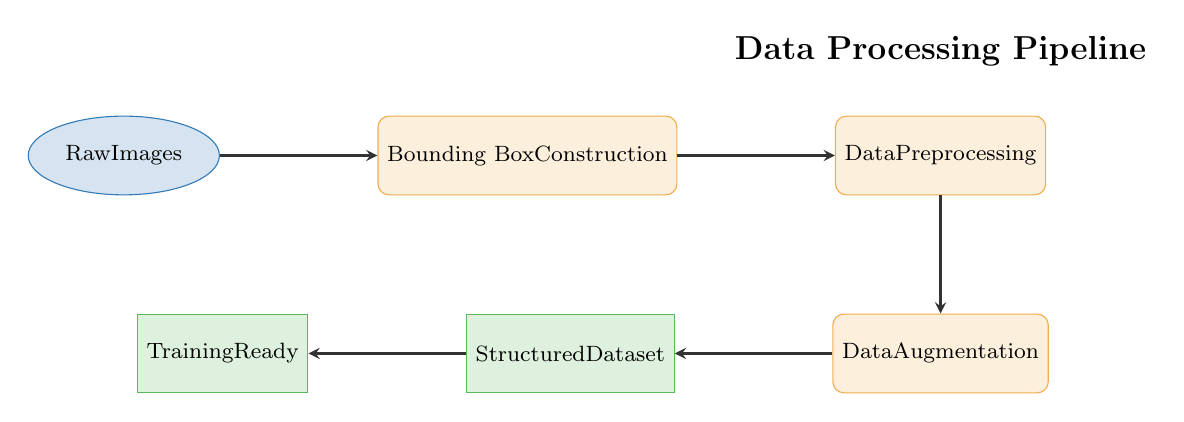
\begin{tikzpicture}[
    node distance=1.5cm and 2cm,
    input/.style={ellipse, minimum width=2cm, minimum height=1cm, text centered, draw=primaryblue, fill=primaryblue!20, font=\footnotesize},
    process/.style={rectangle, rounded corners, minimum width=2.5cm, minimum height=1cm, text centered, draw=warningyellow, fill=warningyellow!20, font=\footnotesize},
    output/.style={rectangle, minimum width=2cm, minimum height=1cm, text centered, draw=successgreen, fill=successgreen!20, font=\footnotesize},
    arrow/.style={thick,->,>=stealth, draw=darkgray}
]

\node (raw_data) [input] {Raw\\Images};
\node (bbox) [process, right=of raw_data] {Bounding Box\\Construction};
\node (preprocessing) [process, right=of bbox] {Data\\Preprocessing};
\node (augmentation) [process, below=of preprocessing] {Data\\Augmentation};
\node (structured) [output, left=of augmentation] {Structured\\Dataset};
\node (training) [output, left=of structured] {Training\\Ready};

\draw [arrow] (raw_data) -- (bbox);
\draw [arrow] (bbox) -- (preprocessing);
\draw [arrow] (preprocessing) -- (augmentation);
\draw [arrow] (augmentation) -- (structured);
\draw [arrow] (structured) -- (training);

\node [above=0.5cm of preprocessing, font=\large\bfseries] {Data Processing Pipeline};

\end{tikzpicture}

% ---
% Figure 8: Production Deployment Architecture
% ---
\begin{tikzpicture}[
    node distance=1.5cm and 2.5cm,
    service/.style={rectangle, rounded corners, minimum width=2.5cm, minimum height=1.2cm, text centered, draw=primaryblue, fill=primaryblue!20, font=\footnotesize},
    database/.style={cylinder, shape border rotate=90, aspect=0.3, minimum width=2cm, minimum height=1.5cm, text centered, draw=successgreen, fill=successgreen!20, font=\scriptsize},
    api/.style={rectangle, rounded corners, minimum width=2cm, minimum height=1cm, text centered, draw=warningyellow, fill=warningyellow!20, font=\scriptsize},
    arrow/.style={thick,->,>=stealth, draw=darkgray},
    bidirectional/.style={thick,<->,>=stealth, draw=darkgray}
]

\node (input_api) [api] at (0,2) {Input\\API};
\node (preprocessing) [service] at (3,2) {Preprocessing\\Service};
\node (inference) [service] at (6,2) {Inference\\Engine};
\node (xai_service) [service] at (9,2) {XAI\\Service};

\node (model_db) [database] at (6,0) {Model\\Repository};
\node (results_db) [database] at (9,0) {Results\\Database};
\node (monitoring) [service] at (3,0) {Monitoring\\& Logging};

\draw [arrow] (input_api) -- (preprocessing);
\draw [arrow] (preprocessing) -- (inference);
\draw [arrow] (inference) -- (xai_service);
\draw [bidirectional] (inference) -- (model_db);
\draw [arrow] (xai_service) -- (results_db);
\draw [arrow] (preprocessing) -- (monitoring);
\draw [arrow] (inference) -- (monitoring);

\node [above=0.5cm of preprocessing, font=\large\bfseries] {Production Deployment Architecture};

\end{tikzpicture}

% ---
% Figure 9: Performance Metrics Dashboard Layout
% ---
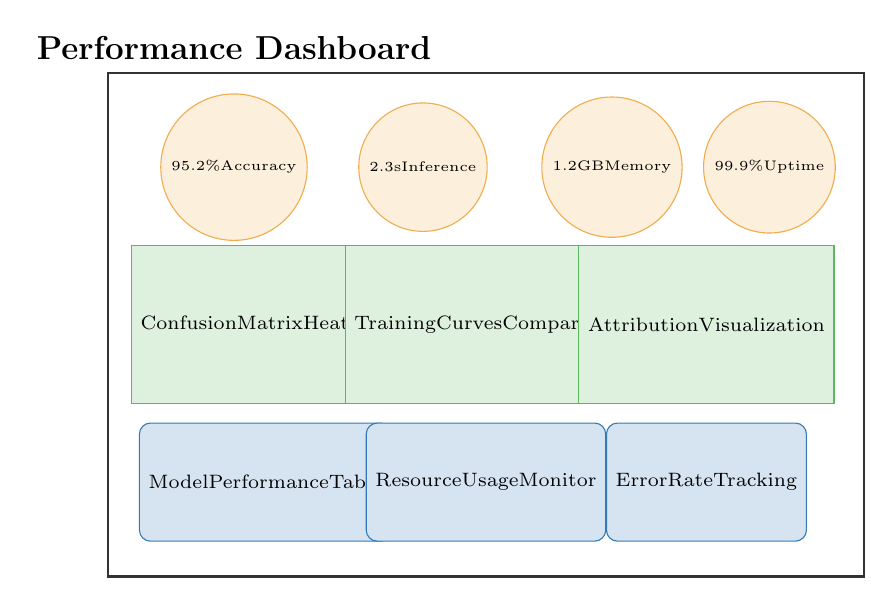
\begin{tikzpicture}[
    scale=0.8,
    metric/.style={rectangle, rounded corners, minimum width=2.5cm, minimum height=1.5cm, text centered, draw=primaryblue, fill=primaryblue!20, font=\scriptsize},
    chart/.style={rectangle, minimum width=3cm, minimum height=2cm, text centered, draw=successgreen, fill=successgreen!20, font=\scriptsize},
    kpi/.style={circle, minimum width=1.5cm, text centered, draw=warningyellow, fill=warningyellow!20, font=\tiny}
]

% Dashboard layout
\draw [thick, darkgray] (0,0) rectangle (12,8);

% KPIs
\node (accuracy_kpi) [kpi] at (2,6.5) {95.2\%\\Accuracy};
\node (speed_kpi) [kpi] at (5,6.5) {2.3s\\Inference};
\node (memory_kpi) [kpi] at (8,6.5) {1.2GB\\Memory};
\node (uptime_kpi) [kpi] at (10.5,6.5) {99.9\%\\Uptime};

% Charts
\node (confusion_matrix) [chart] at (2.5,4) {Confusion\\Matrix\\Heatmap};
\node (training_curves) [chart] at (6,4) {Training\\Curves\\Comparison};
\node (attribution_viz) [chart] at (9.5,4) {Attribution\\Visualization};

% Metrics
\node (performance_table) [metric] at (2.5,1.5) {Model\\Performance\\Table};
\node (resource_usage) [metric] at (6,1.5) {Resource\\Usage\\Monitor};
\node (error_logs) [metric] at (9.5,1.5) {Error\\Rate\\Tracking};

\node [above=0.3cm of accuracy_kpi, font=\large\bfseries] {Performance Dashboard};

\end{tikzpicture}

% ---
% Figure 10: Model Interpretability Framework
% ---
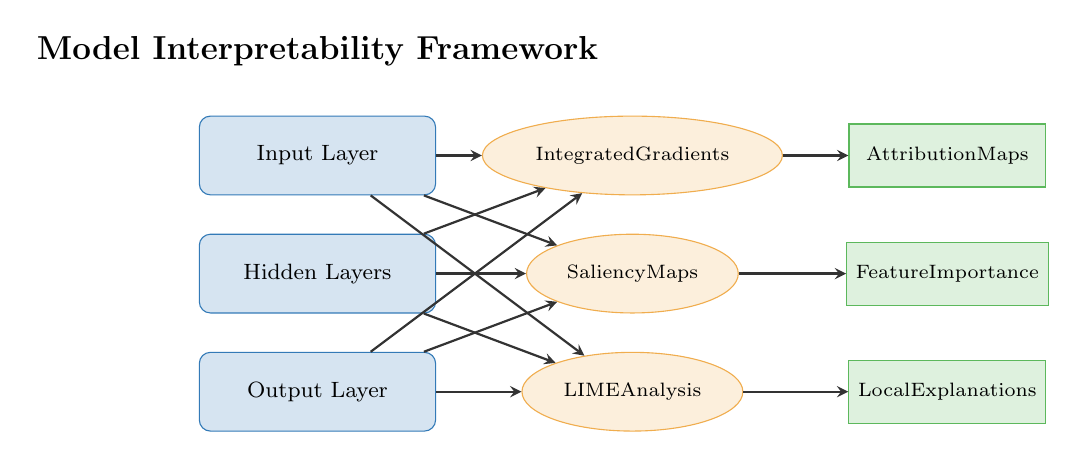
\begin{tikzpicture}[
    node distance=2cm and 2.5cm,
    layer/.style={rectangle, rounded corners, minimum width=3cm, minimum height=1cm, text centered, draw=primaryblue, fill=primaryblue!20, font=\footnotesize},
    technique/.style={ellipse, minimum width=2.5cm, minimum height=1cm, text centered, draw=warningyellow, fill=warningyellow!20, font=\scriptsize},
    output/.style={rectangle, minimum width=2.5cm, minimum height=0.8cm, text centered, draw=successgreen, fill=successgreen!20, font=\scriptsize},
    arrow/.style={thick,->,>=stealth, draw=darkgray}
]

% Model layers
\node (input_layer) [layer] at (0,3) {Input Layer};
\node (hidden_layers) [layer] at (0,1.5) {Hidden Layers};
\node (output_layer) [layer] at (0,0) {Output Layer};

% XAI techniques
\node (integrated_grad) [technique] at (4,3) {Integrated\\Gradients};
\node (saliency) [technique] at (4,1.5) {Saliency\\Maps};
\node (lime) [technique] at (4,0) {LIME\\Analysis};

% Outputs
\node (attribution_maps) [output] at (8,3) {Attribution\\Maps};
\node (feature_importance) [output] at (8,1.5) {Feature\\Importance};
\node (explanations) [output] at (8,0) {Local\\Explanations};

% Arrows
\foreach \layer in {input_layer, hidden_layers, output_layer} {
    \foreach \technique in {integrated_grad, saliency, lime} {
        \draw [arrow] (\layer) -- (\technique);
    }
}

\draw [arrow] (integrated_grad) -- (attribution_maps);
\draw [arrow] (saliency) -- (feature_importance);
\draw [arrow] (lime) -- (explanations);

\node [above=0.5cm of input_layer, font=\large\bfseries] {Model Interpretability Framework};

\end{tikzpicture}

\end{document}
